\documentclass[11pt,fleqn]{article}
%\usepackage{CJK}
\usepackage{latexsym}
\usepackage{color}
\usepackage{graphicx, float}\usepackage{graphicx}
\usepackage{algorithmic}
\usepackage{algorithm}
%\usepackage{algpseudocode}
%\usepackage[colorlinks]{hyperref}
\usepackage[toc,page]{appendix}
\usepackage{bm}
\setlength{\oddsidemargin}{-0.0in}
\setlength{\evensidemargin}{-0.0in} \setlength{\textwidth}{6.0in}
\setlength{\textheight}{9.0in} \setlength{\topmargin}{-0.2in}
%\usepackage[boxruled]{algorithm2e}

%\setlength{\leftmargin}{0.7in}
\usepackage{amssymb, graphicx, amsmath}  %  fancyheadings,
\usepackage{setspace}
\newcommand\qed{\qquad $\square$}
\newcommand{\nn}{\nonumber}

\usepackage{lipsum}

\usepackage{listings}
\lstset{
  basicstyle=\ttfamily,
  columns=fullflexible,
  frameround=fttt,
  breaklines=true,
  %postbreak=\mbox{\textcolor{red}{$\hookrightarrow$}\space},
}

\definecolor{mGreen}{rgb}{0,0.6,0}
\definecolor{mGray}{rgb}{0.5,0.5,0.5}
\definecolor{mPurple}{rgb}{0.58,0,0.82}
\definecolor{backgroundColour}{rgb}{0.95,0.95,0.92}

\lstdefinestyle{CStyle}{
    backgroundcolor=\color{backgroundColour},   
    commentstyle=\color{mGreen},
    keywordstyle=\color{magenta},
    numberstyle=\tiny\color{mGray},
    stringstyle=\color{mPurple},
    basicstyle=\footnotesize,
    breakatwhitespace=false,         
    breaklines=true,                 
    captionpos=b,                    
    keepspaces=true,                 
    numbers=left,                    
    numbersep=5pt,                  
    showspaces=false,                
    showstringspaces=false,
    showtabs=false,                  
    tabsize=2,
    language=C
}

\def \[{\begin{equation}}
\def \]{\end{equation}}
\def\proof{{\bf Proof:\quad}}
\def \endzm {\quad $\Box$}
\def\dist{\hbox{dist}}

\usepackage{tabularx,booktabs}
\newcolumntype{C}{>{\centering\arraybackslash\hsize=.5\hsize}X} % centered version of "X" type
\setlength{\extrarowheight}{1pt}
\usepackage{caption}% <-- added


\newcommand{\R}{\mathbb{R}}
%\newtheorem{yinli}{����}[section]
\newcommand{\D}{\displaystyle}
\newcommand{\T}{\textstyle}
\newcommand{\SC}{\scriptstyle}
\newcommand{\FT}{\footnotesize}

\usepackage{hyperref}
\newcommand\fnurl[2]{%
  \href{#2}{#1}\footnote{\url{#2}}%
}


%\newtheorem{theorem}{Theorem}[section]
%\renewcommand{\thetheorem}{\arabic{section}.\arabic{theorem}}
\newtheorem{definition}{Definition}
\renewcommand{\thedefinition}{\arabic{section}.\arabic{definition}}
\newtheorem{lemma}{Lemma}[section]
\renewcommand{\thelemma}{\arabic{section}.\arabic{lemma}}
\newtheorem{remark}{Remark}
\renewcommand{\theremark}{\arabic{section}.\arabic{remark}}
\newtheorem{proposition}{Proposition}[section]
\renewcommand{\theproposition}{\arabic{section}.\arabic{proposition}}
\newtheorem{corollary}{Corollary }[section]
\renewcommand{\thecorollary}{\arabic{section}.\arabic{corollary}}
\renewcommand{\theequation}{\arabic{section}.\arabic{equation}}
\renewcommand{\baselinestretch}{1.35}
\newtheorem{exam}{Example}[section]
\renewcommand{\theexam}{\arabic{section}.\arabic{exam}}
\newtheorem{theo}{Theorem}[section]
\renewcommand{\thetheo}{\arabic{section}.\arabic{theo}}

% Define a \HEADER{Title} ... \ENDHEADER block
\makeatletter
\newcommand{\HEADER}[1]{\ALC@it\underline{\textsc{#1}}\begin{ALC@g}}
\newcommand{\ENDHEADER}{\end{ALC@g}}
\makeatother

\newcommand{\argmin}{\operatornamewithlimits{argmin}}
\newcommand{\argmax}{\operatornamewithlimits{argmax}}

\usepackage{url} % to make url in bibtex shows up

\begin{document}
%\begin{CJK*}{GBK}{song}

\begin{center}

{\LARGE \bf Measure File Systems' Write Amplification}\\

\vskip 25pt
 {Zeyuan Hu \\ iamzeyuanhu@utexas.edu }\\
\vskip 5pt
%{\small EID:zh4378 Fall 2018 }

\end{center}

\begin{spacing}{1.5}
\section{Introduction}

\noindent In this writeup, we empirically measure the write amplification for file system and
detail the steps to reproduce the said result. 

\section{Background}

We follow the concepts from ``Designing Access Methods: The RUM Conjecture"
\cite{athanassoulis2016designing} to define the space amplification and write amplification. There are two types of
data: base data and auxiliary data. Base data means the main data stored in the system that we want to read or update.
For example, the data to be written into the file system. Auxiliary data represents the data used for performance improvements
on updating of base data. For example, when we append a block of data to a file, file system changes three blocks of data:
the data block itself (base data), the inode block (auxiliary data), and the data bitmap (auxiliary data). Then the write amplification and space amplification can be defined as following:

$$
\text{write amplification} = \frac{\text{update size to the auxiliary data} + \text{update size to the base data}}{\text{update size to the base data}}
$$

$$
\text{space amplification} = \frac{\text{space increase for auxiliary data} + \text{space increase for base data}}{\text{space increase for base data}}
$$

For our appending a block of data to a file example, the write amplification is three because $\text{``update size to the auxiliary data"} = 2$ (the inode block, the data bitmap) and $\text{``update to the base data"}$ is one (the data block). For the space amplification, 
since both updates to the inode block and the data bitmap are overwrite and $\text{``space increase for auxiliary data"} = 0$, thus
both numerator and denominator is one. Thus, the space amplification is one.

\section{Environment}

We use a machine that has 4 Intel(R) Core(TM) i5 CPU @ 3.60GHz processors and 4GB of memory. The machine runs 
Ubuntu 14.04.5 LTS (kernel version 4.8.12). There are one HDD (e.g., \lstinline|/dev/sda1|) and one SSD
(e.g., \lstinline|/dev/sdb1|) in the machine. We will use the SSD to run all of our experiments.

\section{Measure the Write Amplification of file systems using Filebench}

\subsection{Setup the Filebench}

Filebench \cite{tarasov2016filebench} is a file system and storage benchmark that can generate various workloads.
We use Filebench 1.5-alpha3 version to perform our experiments. We first install the Filebench to our environment:

\begin{lstlisting}
$ wget https://github.com/filebench/filebench/releases/download/1.5-alpha3/filebench-1.5-alpha3.tar.gz
$ tar zxvf filebench-1.5-alpha3.tar.gz
$ cd filebench-1.5-alpha3/
$ ./configure --prefix=$HOME/filebench_install
$ make
$ make install
\end{lstlisting}

We run the varmail workload (e.g. \lstinline|varmail.f|) shipped with the Filebench (e.g. \lstinline|filebench_install/share/filebench/workloads|) to measure both the space and the write amplification.
The varmail workload simulates a mail server, which is \lstinline|fsync()| heavy \cite{mohan2017analyzing}. We setup the varmail workload in the same way as
mentioned in ``Analyzing IO Amplification in Linux File Systems" \cite{mohan2017analyzing} paper: 16 threads, total files 100K, mean file size 16 KB.
We modify the \lstinline|varmail.f| as following:

\begin{lstlisting}
set $dir=/home/iamzeyuanhu/hzy/empty
set $nfiles=100k
set $meandirwidth=1000000
set $filesize=cvar(type=cvar-gamma,parameters=mean:16384;gamma:1.5)
set $nthreads=16
set $iosize=1m
set $meanappendsize=16k

define fileset name=bigfileset,path=$dir,size=$filesize,entries=$nfiles,dirwidth=$meandirwidth,prealloc=80

define process name=filereader,instances=1
{
  thread name=filereaderthread,memsize=10m,instances=$nthreads
  {
    flowop deletefile name=deletefile1,filesetname=bigfileset
    flowop createfile name=createfile2,filesetname=bigfileset,fd=1
    flowop appendfilerand name=appendfilerand2,iosize=$meanappendsize,fd=1
    flowop fsync name=fsyncfile2,fd=1
    flowop closefile name=closefile2,fd=1
    flowop openfile name=openfile3,filesetname=bigfileset,fd=1
    flowop readwholefile name=readfile3,fd=1,iosize=$iosize
    flowop appendfilerand name=appendfilerand3,iosize=$meanappendsize,fd=1
    flowop fsync name=fsyncfile3,fd=1
    flowop closefile name=closefile3,fd=1
    flowop openfile name=openfile4,filesetname=bigfileset,fd=1
    flowop readwholefile name=readfile4,fd=1,iosize=$iosize
    flowop closefile name=closefile4,fd=1
  }
}

echo  "Varmail Version 3.0 personality successfully loaded"

run 60
\end{lstlisting}


%
%\begin{figure}
%\centering
%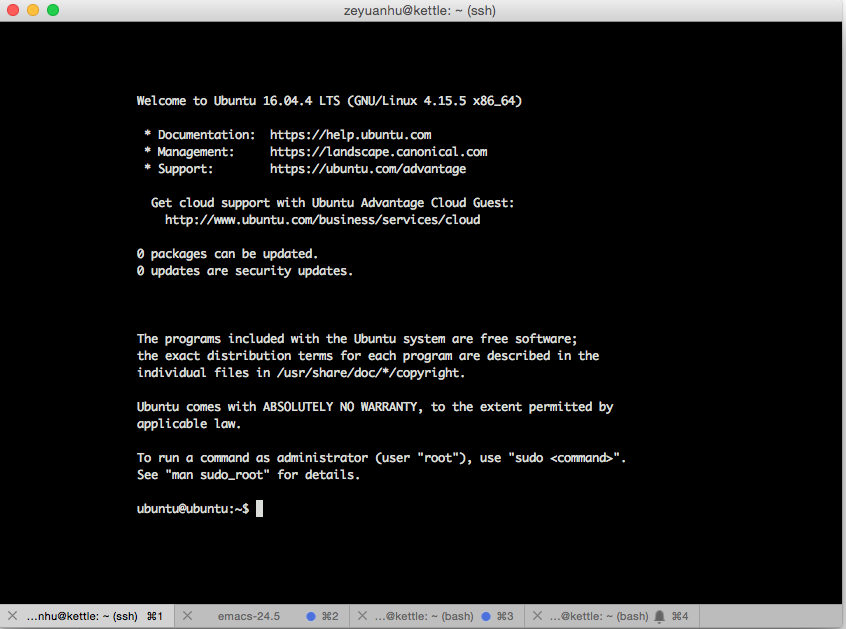
\includegraphics[scale=0.4]{bootup.png} 
%\caption{Login screen of our VM}
%\label{login}
%\end{figure}

\subsection{Way of measurement and the result}

We measure \lstinline|ext2|, \lstinline|ext4|, \lstinline|xfs|, \lstinline|f2fs|, \lstinline|btrfs| mounted on
SSD (e.g. \lstinline|/dev/sdb1|). To calculate the write amplification empirically, we use \texttt{iostat}
\cite{iostat}, \texttt{du} \cite{du}, and \texttt{strace} \cite{strace} along with the customized Filebench.

We modify the Filebench \footnote{https://github.com/xxks-kkk/filebench/tree/amp} to expose two additional statistics:
the total write of the workload and the \texttt{iostat} number difference after the preallocation of the files. As shown
in the varmail workload setup, filebench will initially create a fileset and allocate 80\% of the files before the actual
workload run. Thus, during the calculation of write amplification, we want to exclude the writes done by the preallocation.
We expose the total write of the workload from Filbench because it will give an accurate measure of the number of writes issued
from the workload (i.e., the denominator of the write amplification calculation).

For each file system, we run the command \lstinline|iostat -d /dev/sdb1| first to record \texttt{kB\_wrtn}, which represents
the total number of kilobytes written on the device. Then, we run the filebench and monitor the whole process using the
\texttt{strace}. We filter the \texttt{write} system call. After the finish of the process, we run the \lstinline|iostat -d /dev/sdb1| again to record \texttt{kB\_wrtn} number, calculate the number of bytes
written through the \texttt{write} system call. Then, we
calculate the space and write amplification as following:

$$
\text{write amplification} = \frac{\text{\texttt{kB\_wrtn} number difference} - \text{write done by the preallocation}}{\text{total writes done by the workload}}
$$

%$$
%\text{space amplification} = \frac{\text{space increase for the designated directory}}{\text{total writes through \texttt{write} system call}}
%$$

We automate the whole process through a script \footnote{https://github.com/xxks-kkk/Code-for-blog/blob/master/2018/emmett/filebench/benchmarks/filebench/strace.sh}. The result is shown in Table \ref{result}.


\begin{table}[]
\centering
\begin{tabular}{|l|l|l|l|l|}
\hline
File System & \multicolumn{2}{l|}{Write Amp.}  \\ \hline
Journal On? & Yes             & No             \\ \hline
ext2        & 5.1             & N/A            \\ \hline
ext4        & 4.7             & 3.6            \\ \hline
xfs         & 3.3             & N/A            \\ \hline
f2fs        & 2.4             & N/A            \\ \hline
btrfs       & 5.7             & N/A            \\ \hline
\end{tabular}
\caption{Write amplification for different file systems on SSD \label{result}. We measure whether journaling will cause a significant
incrase in the write amplification of the file system.}
\end{table}

\section{Measure the Write Amplification of file systems using Git-benchmark}

Betrfs \cite{jannen2015betrfs} uses a Git benchmark, which is described in the ``File Systems Fated for Senescence? Nonsense, Says Science!" \cite{conway2017file}. Essentially, the benchmark clones
the Linux repository and perform \texttt{git pull} to patch the code for a fixed amount of times. We're interested to see the amount of data written to the disk shown by the \texttt{iostat}. 

We modified the Git benchmark to include \texttt{sync} after each pull and use \texttt{fstrim} to trim SSD during the inital file system setup. 
We perform 20 pulls for the experiment \footnote{Code: https://github.com/xxks-kkk/Code-for-blog/tree/master/2018/emmett/filebench/benchmarks/git-benchmark}. The result is shown in Table \ref{result2}.

\begin{table}[]
\centering
\begin{tabular}{|l|l|l|}
\hline
File System & \multicolumn{2}{l|}{\texttt{iostat} difference (KB)} \\ \hline
Journal On? & Yes                              & No                             \\ \hline
ext4        & 3277472                          & 3272320                            \\ \hline
\end{tabular}
\caption{The number of KB written to the disk measured by \texttt{iostat} on ext4 \label{result2}}
\end{table}

\end{spacing}

\bibliographystyle{ieeetr}
\bibliography{report}


\end{document}

